\subsection{Dynamic Tension System}
\subsubsection{What is a Dynamic Tension System?}
The dynamic tension system is contained within the front module of Cyclone and ensures that changes in the track tension due to the motion of the suspension are sufficiently counteracted. This  avoids failure due to track derailment. Each track’s tension is independently controlled which is imperative for crossing rough, uneven terrain. \par
Each system consists of a pillow block, two springs, two rods and four spring caps. The front axles, onto which the wheels are fixed, are then placed through the pillow blocks to complete the dynamic tension system seen in figure \ref{fig:DTEN}. The system is held in place by linear bearings which are bolted to the bulkhead, connecting the front module to the centre module. The rods, which are inside the springs, pass through these bearings and are then able to move freely, in a linear motion to enable the system to perform its functionality of providing tension to the tracks. The system is installed in such a way that it will work in conjunction with, but in a reverse manner to  the suspension. When the suspension is compressed, the dynamic tensioning springs will extend to remove the slack produced, by pushing the axle forward, and vice versa. This system will lower the risk of track failure whilst the robot is in operation and thus avoid the manual collection of Cyclone by rescue personnel from potentially hazardous environments. \par
\begin{figure}[h]
\centering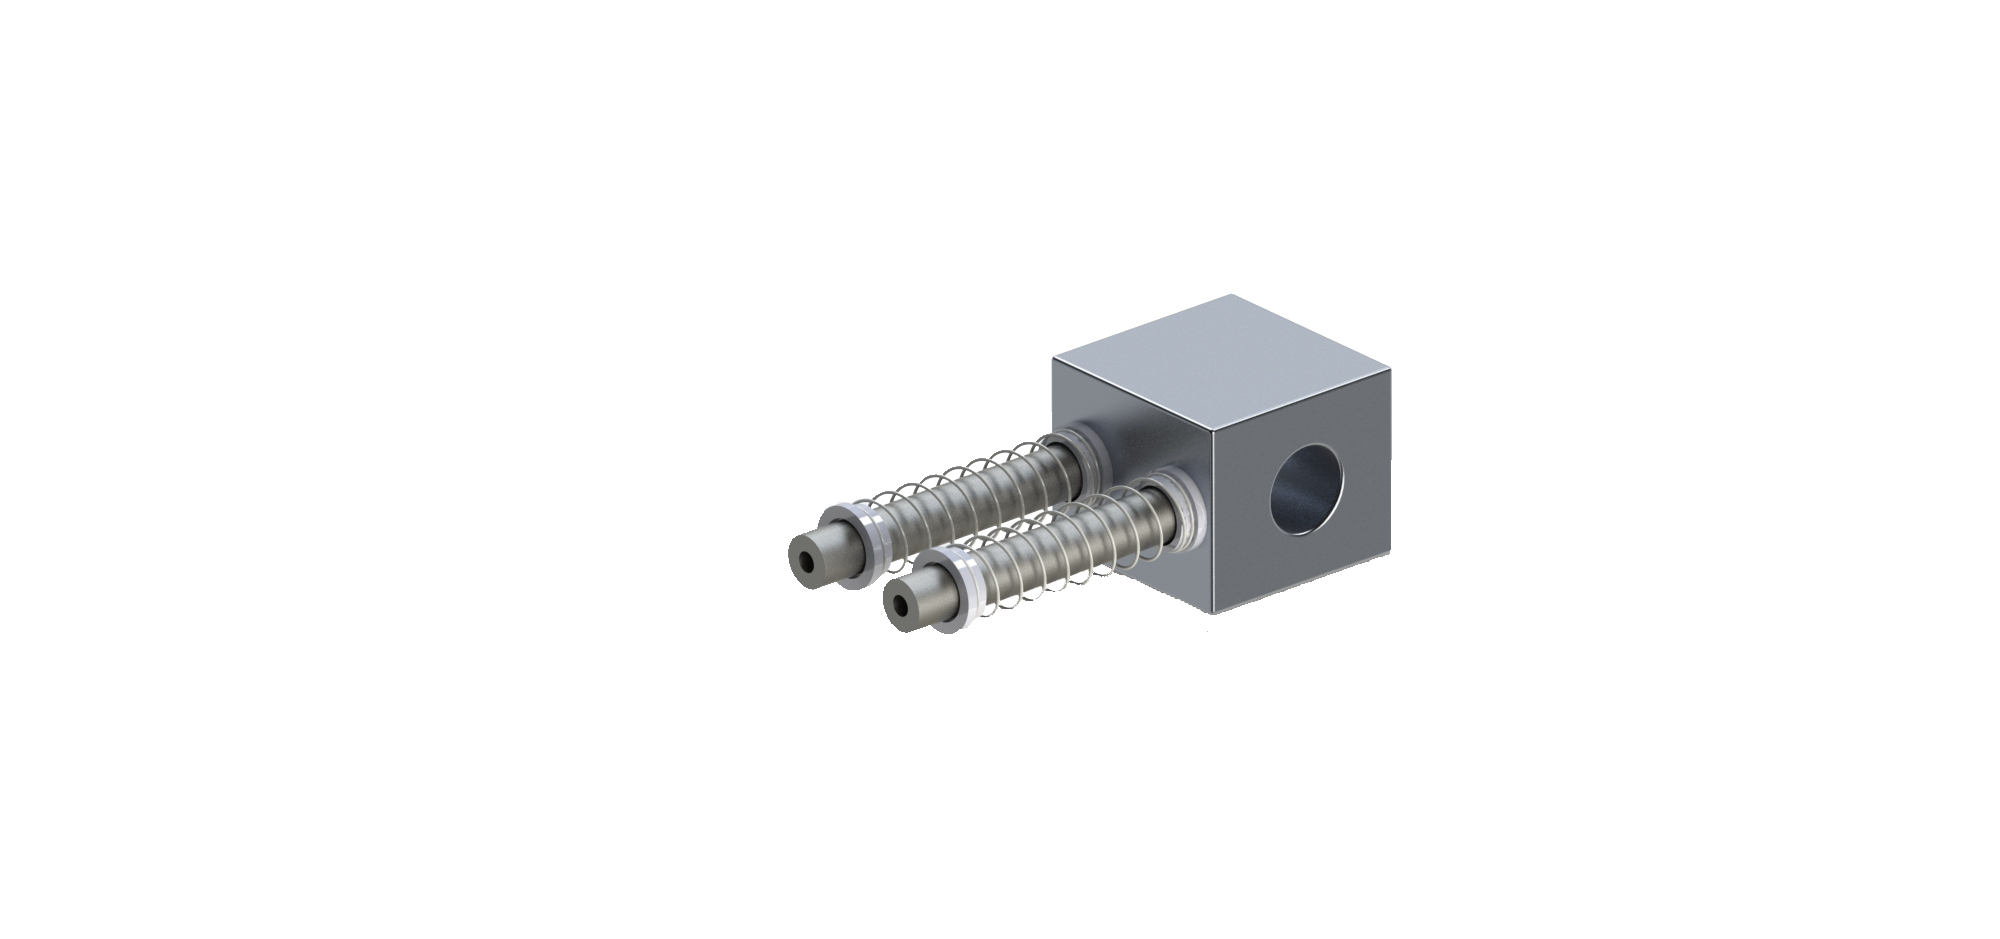
\includegraphics[width=0.8\linewidth]{Images/DTEN_render_1_spring.png}
\caption{Cyclone's Dynamic Tension System Assembly}
\label{fig:DTEN}
\end{figure}
\subsubsection{Analysis of Orion's System}
Orion (2014/15 WMR robot) used a static tensioning system  to alter the tension in the tracks by means of an adapted screw used to locate the pillow blocks in order to tension the tracks. Although simplistic and therefore easy to design and implement, the static nature of this design means that it is not practical for it’s intended purpose (to tension the tracks whilst in motion). During operation, if Orion’s suspension contracted in order to traverse an uneven surface, there would be a high risk of the tracks derailing from the wheels as there is no system in place to reduce this slack whilst the robot is in motion. \par
\subsubsection{Design for Cyclone's System}
As aforementioned, Cyclone will use a dynamic tensioning system. The decision was made to adapt the static system from the previous design to allow dynamic functionality. This allows for the reuse of many of the original components from the previous years design, keeping the design simple and saving on time for both design and manufacture. Springs were chosen as the method of applying a force to the pillow blocks to push the front axles forward so to tension the tracks.  This was found to be the simplest way to provide a force and is easy to implement into the design adapted from the previous year. \par
In order to fully adapt the previous design to that of Cyclones, its faults had to be corrected. This was namely the poor selection of bearings. The linear bearings in the pillow blocks of Orion were replaced with rotational bearings more suited to the rotational motion of the axles. Linear bearings were also used in the bulkhead to allow for the smooth movement of the rods. \par
During design, it was discovered that there was the risk of beaching if the dynamic tensioning system contracted too far, therefore exposing the frame of the robot (ADD FIGURE). To avoid this, the frame was altered to give a shallower profile and a simple stopper was installed in the front module to prevent the springs from contracting too far. \par
IMAGES OF THE BEACHING AND CORRECTIONS. \par
In order to decipher which type of spring was required, specifications had to be identified. The main requirement is that the total spring rate of the systems must not be larger than that of the suspension so that they are not preventing the suspension from performing its own function. Therefore, the spring rate for each of the four springs (two per track) needed to be less than 0.1829 N/mm since this is the value calculated from the suspension. The second requirement is that the springs should allow for the same amount of travel as the suspension to ensure the track tension does not suffer as a result. The maximum travel for the suspension is calculated to be 34mm, and therefore the travel of the dynamic tensioning systems will be at least 34mm. It was advised by the manufacturers that the springs must not be compressed by greater than 80\% of its total length for a continuous period as this will affect its performance. Due to the confined space within which the dynamic tensioning system is located, the free length of the springs is also a factor, this length is limited to 64mm as seen in (ADD IMAGE). The springs also require an inner diameter larger than 10mm (the rod diameter). \par
There was a limited availability of springs that fit these requirements. However, after consultation with Lee Spring, two different types of spring were chosen, seen in table \ref{tab:springparas}. This allowed for testing of both springs and ultimately the (WHICH SPRING WAS CHOSEN?) spring was chosen for the dynamic tensioning. \par
\begin{table}[h]
\centering
\begin{tabular}{|c|c|c|}
\hline
& \multicolumn{2}{|c|}{\textbf{Spring Type}} \\
\hline
Parameters & LP 032K 06 S316 & LP 029K 06 S316 \\
\hline
Outside Diameter (mm) & 13.716 & 13.716 \\
Inside Diameter (mm) & 12.904 & 12.980 \\
Wire Diameter (mm) & 0.812 & 0.736 \\
Free Length (mm) & 50.800 & 50.800 \\
Closed Length (mm) & 10.718 & 8.737 \\
Recommended Travel (mm) & 32.066 & 33.650 \\
Spring Rate (N/mm) & 0.170 & 0.130 \\
\hline
\end{tabular}
\caption{Parameters of Spring Choices}
\label{tab:springparas}
\end{table}
